\begin{figure}[!b]
\begin{center}
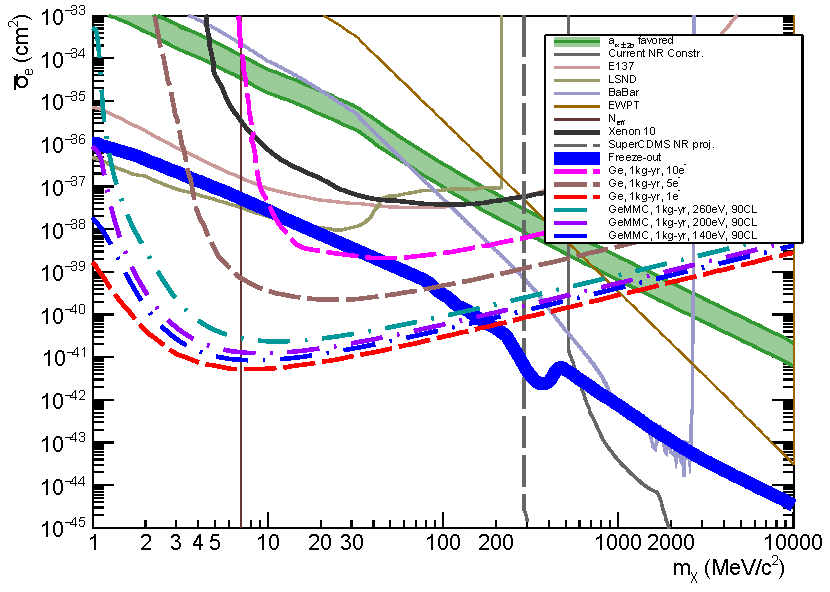
\includegraphics[scale=1]{./fig/DMElektronStreuung.pdf}
\vspace{-0.5cm}
\caption{Sensitivitätskurve für einen DM-Formfaktor FDM = 1 in Kombination
mit Ausschlusskurven anderer Experimente für den DELight Detektor. Die dicke blaue
Linie stellt den durch Freeze-out favorisierten Parameterbereich da.\cite{Lukwata2017}}
\label{fig:DMES}
\end{center}
\end{figure}

Trotz großem experimentellem Aufwand konnte bisher kein eindeutiges WIMP Signal beobachtet werden.
Der theoretisch motivierte Parameterbereich \ac{LDM} von $\SI{}{\mega\electronvolt}\--\SI{}{\giga\electronvolt}$ ist allerdings noch weitgehend unerforscht.
Ziel des DELight Experiments ist es die Sensitivität im Massenbereich von $\SI{1}{\mega\electronvolt}\--\SI{10}{\mega\electronvolt}$ um mehrere Größenordnungen zu verbessern.
Um dieses zu erreichen wird das Ionisationssignal weniger Elektronen einer DM-Elektron Streuung betrachtet\cite{Essig2016}.
Als Target wird Germanium verwendet, welches sich aufgrund seiner geringen effektiven Bandlücke von $\SI{3}{\electronvolt}$ besonders gut eignet.\cite{Essig2012}
Neben Neutrinos ist der Untergrund weitgehend unbekannt.
Eine wichtige Methode um Signal vom Untergrund zu unterscheiden ist die jährliche Modulation des Flusses an DM aufgrund der relativen Geschwindigkeit zwischen dem DM Halo und der Erde\cite{Drukier1986}.
Allerdings gibt es für Signale, wie sie von LDM erwartet werden, kaum Untergrund.
In Abb. \ref{fig:DMES} ist die erwartete Sensitivität des GeMMC Detektors für eine untergrundfreie Exposition von $\SI[inter-unit-product = \cdot]{1}{\kilogram\year}$ dargestellt.

